%! Author = mackesmilian
%! Date = 01.11.21

% Preamble
\documentclass[11pt]{article}
%\addbibresource{../main.bib}
\usepackage{graphicx}
\usepackage[english]{babel}
\usepackage[nottoc]{tocbibind}
\graphicspath{ {/home/mackesmilian/Documents/FH/BACC/bachelorarbeit/src/images/} }
\title{
        {Development and Deployment of Web Applications as Installable Desktop Applications Using
    Electron Framework}\\
    {\large FH Campus 02}\\
}
\author{Maximilian Martin Wolf}
\date{30 October 2021}
% Document
\begin{document}

    \maketitle
    \pagebreak
    \tableofcontents
    \pagebreak


    \section{Introduction}\label{sec:introduction}
    \setcounter{tocdepth}{3}

    \subsection{What Is Electron?}\label{subsec:what-is-electron}
    In December 2012 software engineer Cheng Zhao joined GitHub's team, having previously worked for Intel developing
node-webkit, with the task of porting the Atom editor from using Chromium Embedded Framework to node-webkit.
Node-webkit being a Node.js module developed by Roger Wang which combined the browser engine used by Chromium - WebKit - 
with Node.js, making Node.js modules accessible from JavaScript code running inside a web page. \parencite{jensen2017}\paragraph{}

Porting to node-webkit proved difficult, so GitHub abandoned that approach, and it was decided that a new native shell
for Atom would be created.
Said shell was dubbed \emph{Atom Shell} and after development was finished and the Atom editor was open sourced
by GitHub, Atom Shell soon followed suit and was renamed to \emph{Electron}.
Initially developed as a way to deliver an editor, numerous widely known applications like Slack, Discord and Visual
Studio have started using Electron to develop and deliver their desktop applications.\parencite{electronDocs}
But what exactly is Electron?\paragraph{}
Electron is a framework which allows for the development of cross-platform desktop applications using only popular 
web programming languages like HTML, CSS and JavaScript. 
While the advantages will be discussed in detail in the next chapter \emph{Why Use Electron?}, the appeal to developers
is obvious: Maintaining one codebase while being able to deliver the app to all desktop operating systems.\paragraph{}
Now, as described previously the Electron framework serves the same purpose as node-webkit (later renamed to NW.js), but
their approaches do differ in certain ways: \parencite{jensen2017}\par
\begin{figure}[ht]
    \label{fig:el-architecture}
    \caption{A simplified representation of Electron's architecture. \parencite{jensen2017}}
    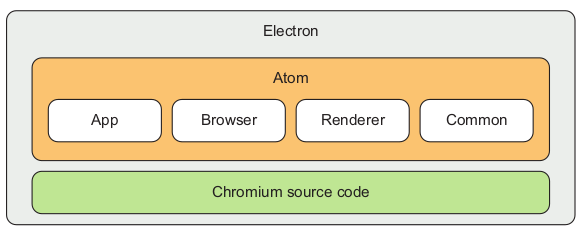
\includegraphics[width=\textwidth]{electron-architecture}
\end{figure}
Without going into detail on how NW.js works, Electron and NW.js share some architectural similarities.
However, there are some differences in how Electron combines Node.js with Chromium.\paragraph{}
Architecturally, Electron places an emphasis on strict separation from Chromium source code, ass seen in figure \ref{fig:el-architecture}.
This looser integration allows for easier updates to the Chromium part of the source code, whereas with NW.js Chromium
is patched to allow for Node.js and Chromium to use a shared Javascript state. \parencite{jensen2017}\par
On the other hand, this means that Electron has separate JavaScript contexts: A \emph{main} process which starts running
with the app window and a \emph{renderer} process for each individual window.
Any sharing of state between these contexts, or simply put between the front- and back-end, has to pass through the
\emph{icpMain} and \emph{icpRenderer} modules.
This means that each JavaScript context is kept separate but data can be explicitly shared, allowing for greater control
over what state exists in which app window. \parencite{jensen2017}\paragraph{}
Electron itself (the part without Chromium) is made up of for different components: App, Browser, Renderer and Common.
\textbf{App} contains code written in C++ and Objective-C++ responsible for loading Node.js and Chromium's content module.
The \textbf{browser} folder contains code which handles interactions with the front-end.
This is to say functionality such as loading the JavaScript engine, interacting with the UI and binding operating system
specific modules.
As for \textbf{renderer}, this component handles the different renderer processes.
Because Chromium works by running each tab as an individual process, as to not crash the entire browser should one
tab become unresponsive, each application window in Electron runs as its own process.
\textbf{Common} contains code which is used by both the main and renderer processes for running the application.
Among other things this folder also contains the integration of Node.js' event loop with Chromium's event loop. \parencite{jensen2017}\paragraph{}


    \subsection{Why Use Electron?}\label{subsec:why-use-electron}
    Now the next obvious question is why a framework such as Electron is needed at all.
After all, it is "just" a way to have desktop applications developed using HTML, CSS and JavaScript.
So why not just develop native desktop applications or traditional web applications depending on the use case?
To answer this one has to examine the bigger picture:\paragraph{}
Over the past decade it seems as though software pricing has moved from perpetual licenses towards subscription-based
models.
If one examines the data regarding end-user spending on cloud applications it is clear that the
\emph{Software as a Service} (SaaS) model has grown considerably in revenue and is projected to do so in the future:
The worldwide end user spending for Software as a Service has increased from 31.4 billion US Dollars in 2015 to 120
billion US Dollars in 2020.
It is projected this growth will progress with spending reaching 171.9 billion dollars in 2022. \parencite{gartner2021}\paragraph{}
Furthermore, \textcite{gartner2021} forecasts that by 2026, cloud spending will exceed 45\% of all enterprise IT spending, up from
17\% in 2021.
This impressive growth can be attributed to two reasons.
Reasons either technical and/or financial in nature.
One financial benefit of SaaS is economies of scale:
By hosting the application centrally and by extension aggregating users together, providers can benefit financially from
leveraging economies of scale.
At the simple end, this means benefiting from volume pricing on hardware such as data centers, servers, space and so on.
Taking this idea further, SaaS providers can also cut costs by sharing hardware across their customers.
It is not cost-effective to use one machine for each customer, instead resources should be shared and dynamically
allocated on-demand to each customer's needs.
Similarly, as user count increases, the cost of adding on single user decreases.
These and other reasons are a big financial motivator for providers of software to switch to the SaaS model.\paragraph{}
However, technological reasons play a large role as well.
According to \textcite{jacobs2005} the ever-increasing maturity of the Web is a major contributor for the rise in popularity of
SaaS.\par
Browsers are significantly more powerful than ever. 
The \emph{browser wars} of the mid-to-late nineties started with Microsoft and Netscape outdoing each other with
new features, faster and overall better browsers leading to significant leaps in browser technology. \parencite{mozilla2021,jensen2017}\paragraph{}
Furthermore, internet access is more widespread than ever.
In the United States, the number of internet users rose from 229,91 million in 2010 to 302,28 million in 2021,
which constitutes a 31\% increase.\par
\begin{figure}[H]
    \centering
    \label{fig:num-of-internet-users}
    \caption{Number of internet users in the US from 2010 to 2025. \parencite{statista2021}}
    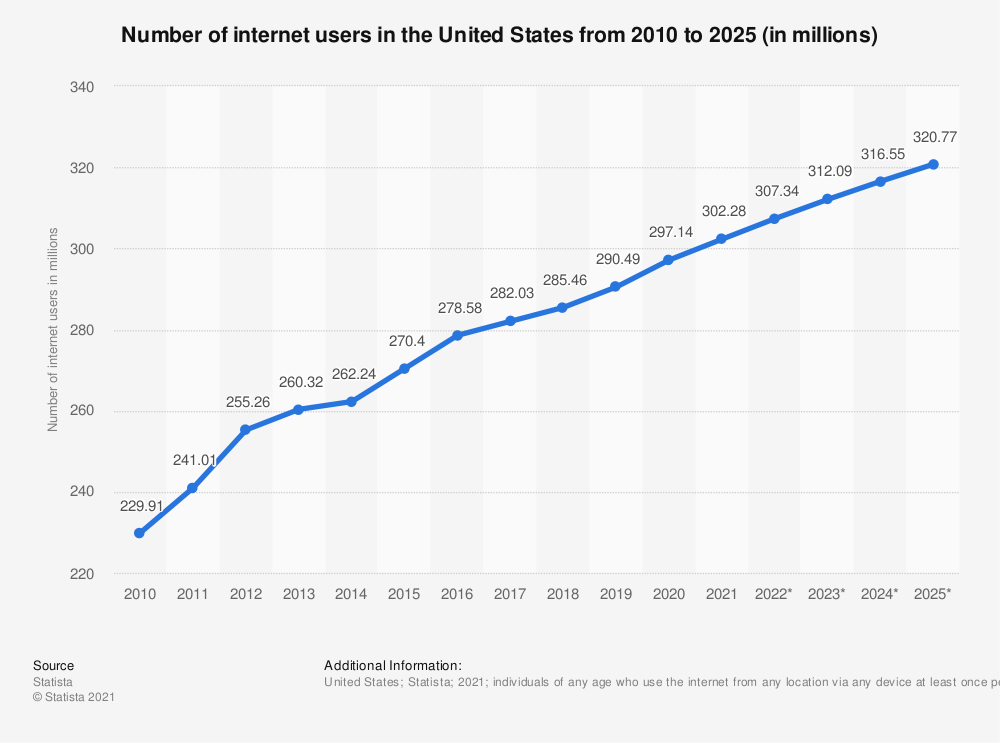
\includegraphics[width=0.8\textwidth]{number-of-internet-users}
\end{figure}
And not only have the number of internet users risen over the past eleven years, the average connection speed increased as well
over the same time period:
\begin{figure}[H]
    \centering
    \label{fig:internet-speed}
    \caption{Average internet connection speed in the US 2007-2017. \parencite{akamai2017}}
    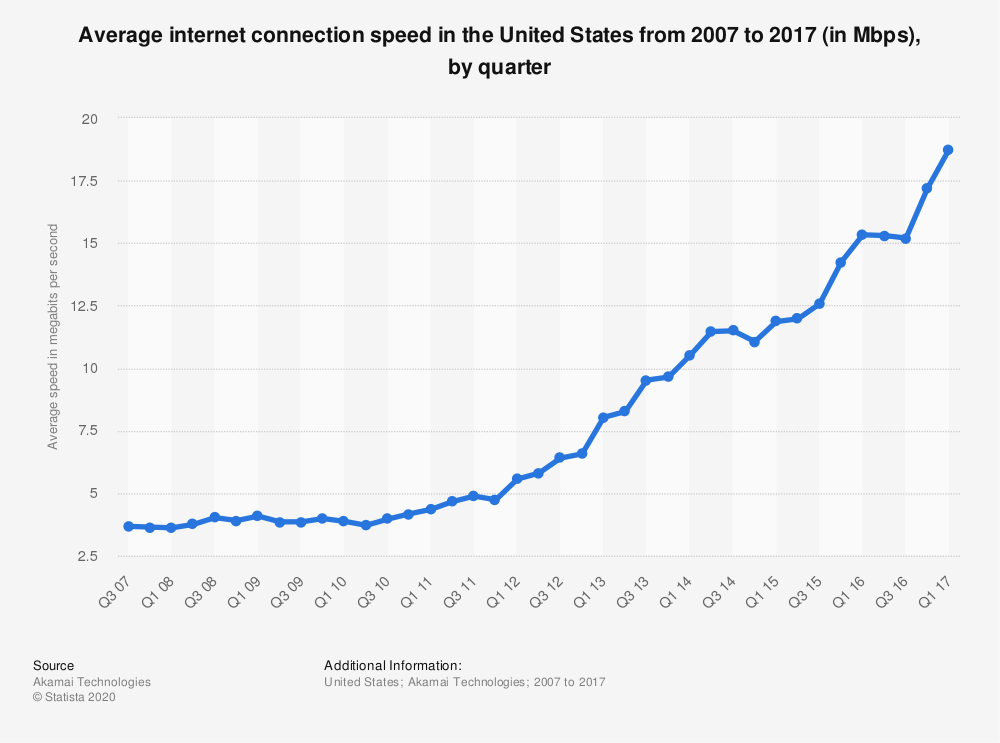
\includegraphics[width=0.8\textwidth]{internet-connection-speed}
\end{figure}
As seen above, from Q3 2017 to Q1 2017, average internet speeds across the US rose by 410\%.
This allowed for much more elaborate websites where larger amounts of data have to be downloaded.
Moreover, the number of robust frameworks for web development (be it front-end or back-end), make creating a complex web application easier
than ever before.
However, while this explains why SaaS is often the billing model of choice, it doesn't fully explain why specifically web applications
have risen in popularity. \parencite{statista2021}\par
After all, SaaS can also be delivered as a Desktop Application, as seen with the Adobe Creative Suite for example. \parencite{adobe2021}\par
To answer this, one should examine how desktop applications and web applications differ in more detail.



    \subsubsection{Desktop Applications}\label{subsubsec:desktop-applications}

    \subsubsection{Web Applications}\label{subsubsec:web-applications}

    \subsubsection{Electron as a Solution}\label{subsubsec:electron-as-solution}


    \section{Method}\label{sec:method}

    \subsection{Developing with Electron}\label{subsec:developing-with-electron}

    \subsubsection{Requirements Analysis}\label{subsubsec:dev-requirements}

    \subsubsection{Development Workflow with Electron}\label{subsubsec:dev-workflow}

    \subsubsection{Finished Project}\label{subsubsec:dev-project}


    \section{Analysis}\label{sec:analysis}

    \subsection{Results}\label{subsec:results}

    \subsection{Vaadin as an Alternative to Electron}\label{subsec:vaadin-electron}
    \bibliographystyle{apa}
    \bibliography{main}
    \pagebreak
    \listoffigures

\end{document}